\PassOptionsToPackage{table,dvipsnames,svgnames}{xcolor}
\documentclass[a0paper,portrait]{baposter}

\usepackage{wrapfig}
\usepackage{lmodern}
\usepackage{amsfonts}
\usepackage{amsmath}
\usepackage{amsthm}
\usepackage{multicol}
\usepackage{hyperref}
\usepackage{subcaption}
\usepackage[utf8]{inputenc}
\usepackage[T1]{fontenc}

\usepackage{graphicx}
\usepackage{tikz}
\usetikzlibrary{positioning}
\usetikzlibrary{shapes}
\usetikzlibrary{shapes.geometric}
\usetikzlibrary{fit}
\usetikzlibrary{calc}

\selectcolormodel{cmyk}
\usepackage{xcolor}

\graphicspath{{figures/}}

\newcommand{\compresslist}{%
\setlength{\itemsep}{0pt}%
\setlength{\parskip}{1pt}%
\setlength{\parsep}{0pt}%
}

\newcommand{\argmax}{\arg\!\max}
\newenvironment{boenumerate}
  {\begin{enumerate}\renewcommand\labelenumi{\textbf\theenumi.}}
  {\end{enumerate}}

\begin{document}

\selectcolormodel{RGB}
\definecolor{darkred}{RGB}{140, 16, 16}
\definecolor{lightred}{RGB}{104, 2, 2}

\begin{poster}
{
grid=false,
headerborder=open, % Adds a border around the header of content boxes
colspacing=1em, % Column spacing
bgColorOne=white, % Background color for the gradient on the left side of the poster
bgColorTwo=white, % Background color for the gradient on the right side of the poster
borderColor=darkred, % Border color
headerColorOne=lightred, % Background color for the header in the content boxes (left side)
headerColorTwo=lightred, % Background color for the header in the content boxes (right side)
headerFontColor=white, % Text color for the header text in the content boxes
boxColorOne=white, % Background color of the content boxes
textborder=rounded, %rectangle, % Format of the border around content boxes, can be: none, bars, coils, triangles, rectangle, rounded, roundedsmall, roundedright or faded
eyecatcher=false, % Set to false for ignoring the left logo in the title and move the title left
headerheight=0.11\textheight, % Height of the header
headershape=rounded, % Specify the rounded corner in the content box headers, can be: rectangle, small-rounded, roundedright, roundedleft or rounded
headershade=plain,
headerfont=\Large\textsf, % Large, bold and sans serif font in the headers of content boxes
%textfont={\setlength{\parindent}{1.5em}}, % Uncomment for paragraph indentation
linewidth=2pt, % Width of the border lines around content boxes
columns=6
}
{}
%
%----------------------------------------------------------------------------------------
%	TITLE AND AUTHOR NAME
%----------------------------------------------------------------------------------------
%
{
\textsf %Sans Serif
{End-To-End Imitation Learning of Lane Following Policies Using Sum-Product Networks
}
}
{\sf\vspace{0.01em}\\
Renato Lui Geh, Denis Deratani Mauá
\vspace{0.1em}\\
\small{Department of Computer Science, Institute of Mathematics and Statistics, University of São
  Paulo, Brazil
\vspace{0.2em}\\
\{renatolg,ddm\}@ime.usp.br}
}
{\includegraphics[scale=0.14]{ime.pdf}} % University/lab logo
\headerbox{1. Task}{name=task,column=0,row=0, span=6}{
  \begin{center}
    \begin{minipage}{0.98\textwidth}
      \begin{minipage}{0.4\textwidth}
        \begin{description}
          \item[Task:] Complete whole course without going off track.
          \item[Input:] Single frontal camera image.
          \item[Output:] Policy $\pi$ with probabilities of actions.
          \item[Actions:] Turn left, right or go straight.
        \end{description}
      \end{minipage}
      \begin{minipage}{0.6\textwidth}
          \includegraphics[width=0.475\textwidth]{demo_merged_pairs_small.png}
          \includegraphics[width=0.475\textwidth]{track_1_resize.png}
      \end{minipage}
    \end{minipage}
  \end{center}
}
\headerbox{2. Sum-Product Networks}{name=spn,span=2,column=0,below=task}{
  \begin{center}
    \begin{minipage}[t][8.25cm]{0.98\textwidth}
      Sum-product networks (SPNs) are deep tractable density estimators with a neural network-like
      structure subject to only sums and products as activation functions.
      \begin{center}
        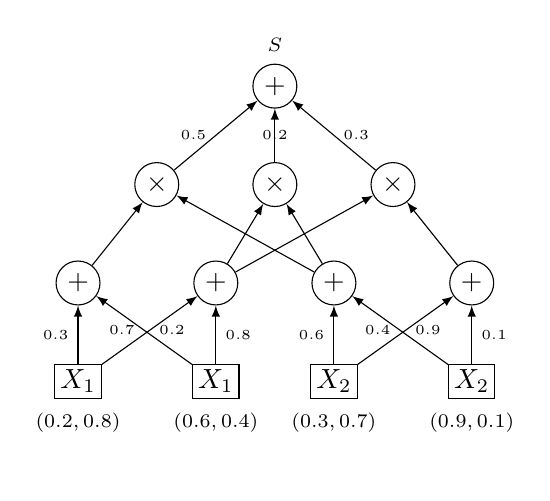
\begin{tikzpicture}
          \begin{scope}[every node/.style={circle,draw,inner sep=2pt}]
            \node[label={[label distance=0pt]above:\scriptsize$S$}] (root) at (0, 0) {$+$};
            \node (p1) at (-1.5, -1.25) {$\times$};
            \node (p2) at (0, -1.25) {$\times$};
            \node (p3) at (1.5, -1.25) {$\times$};
            \node (s1) at (-2.5, -2.5) {$+$};
            \node (s2) at (-0.75, -2.5) {$+$};
            \node (s3) at (0.75, -2.5) {$+$};
            \node (s4) at (2.5, -2.5) {$+$};
            \node[draw,fill=none,rectangle,label={[label distance=-10pt]below:\scriptsize$(0.2, 0.8)$}] (x11) at (-2.5, -3.75) {${X}_1$};
            \node[draw,fill=none,rectangle,label={[label distance=-10pt]below:\scriptsize$(0.6, 0.4)$}] (x12) at (-0.75, -3.75) {${X}_1$};
            \node[draw,fill=none,rectangle,label={[label distance=-10pt]below:\scriptsize$(0.3, 0.7)$}] (x21) at (0.75, -3.75) {${X}_2$};
            \node[draw,fill=none,rectangle,label={[label distance=-10pt]below:\scriptsize$(0.9, 0.1)$}] (x22) at (2.5, -3.75) {${X}_2$};
          \end{scope}
          \begin{scope}[every path/.style={->},>=latex]
            \draw (p1) -- node[left]{\tiny$0.5$} (root);
            \draw (p2) -- node{\tiny$0.2$} (root);
            \draw (p3) -- node[right]{\tiny$0.3$} (root);
            \draw (s1) -- (p1);
            \draw (s3) -- (p1);
            \draw (s2) -- (p2);
            \draw (s3) -- (p2);
            \draw (s2) -- (p3);
            \draw (s4) -- (p3);
            \draw (x11) -- node[left]{\tiny$0.3$} (s1);
            \draw (x12) -- node[left]{\tiny$0.7$} (s1);
            \draw (x11) -- node[right]{\tiny$0.2$} (s2);
            \draw (x12) -- node[right]{\tiny$0.8$} (s2);
            \draw (x21) -- node[left]{\tiny$0.6$} (s3);
            \draw (x22) -- node[left]{\tiny$0.4$} (s3);
            \draw (x21) -- node[right]{\tiny$0.9$} (s4);
            \draw (x22) -- node[right]{\tiny$0.1$} (s4);
          \end{scope}
        \end{tikzpicture}
      \end{center}
      \vspace{-0.5cm}
      In the above example, leaves are binomial distributions over each RV $X_i$.
    \end{minipage}
  \end{center}
}
\headerbox{3. Inference in SPNs}{name=inf,span=2,column=2,below=task}{
  \begin{center}
    \begin{minipage}[t][8.25cm]{0.98\textwidth}
      The probability of evidence of
      \vspace{-0.2cm}
      \begin{center}
        $\mathbf{e}=\{X_1=1,X_2=0\}$
      \end{center}
      \vspace{-0.2cm}
      is the value of the SPN's root.
      \vspace{-0.3cm}
      \begin{center}
        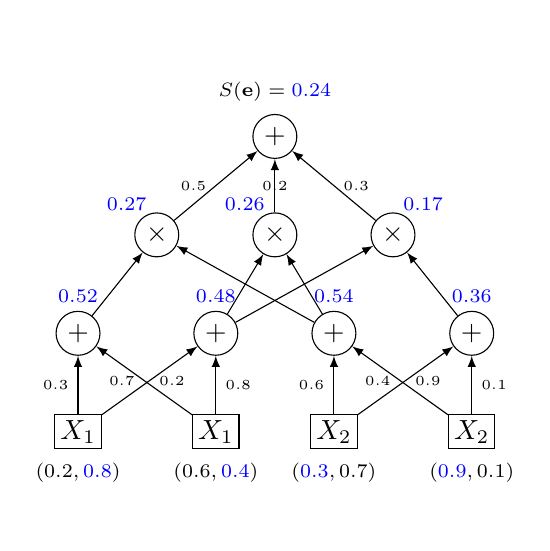
\begin{tikzpicture}
          \begin{scope}[every node/.style={circle,draw,inner sep=2pt}]
            \node[label={[label distance=-15pt]above:\scriptsize$S(\mathbf{e})=\textcolor{blue}{0.24}$}] (root) at (0, 0) {$+$};
            \node[label={[label distance=-3pt]above left:\scriptsize$\textcolor{blue}{0.27}$}] (p1) at (-1.5, -1.25) {$\times$};
            \node[label={[label distance=-3pt]above left:\scriptsize$\textcolor{blue}{0.26}$}] (p2) at (0, -1.25) {$\times$};
            \node[label={[label distance=-3pt]above right:\scriptsize$\textcolor{blue}{0.17}$}] (p3) at (1.5, -1.25) {$\times$};
            \node[label={[label distance=-5pt]above:\scriptsize$\textcolor{blue}{0.52}$}] (s1) at (-2.5, -2.5) {$+$};
            \node[label={[label distance=-5pt]above:\scriptsize$\textcolor{blue}{0.48}$}] (s2) at (-0.75, -2.5) {$+$};
            \node[label={[label distance=-5pt]above:\scriptsize$\textcolor{blue}{0.54}$}] (s3) at (0.75, -2.5) {$+$};
            \node[label={[label distance=-5pt]above:\scriptsize$\textcolor{blue}{0.36}$}] (s4) at (2.5, -2.5) {$+$};
            \node[draw,fill=none,rectangle,label={[label distance=-10pt]below:\scriptsize$(0.2,
              \textcolor{blue}{0.8})$}] (x11) at (-2.5, -3.75) {${X}_1$};
            \node[draw,fill=none,rectangle,label={[label distance=-10pt]below:\scriptsize$(0.6,
              \textcolor{blue}{0.4})$}] (x12) at (-0.75, -3.75) {${X}_1$};
            \node[draw,fill=none,rectangle,label={[label
              distance=-10pt]below:\scriptsize$(\textcolor{blue}{0.3}, 0.7)$}] (x21) at (0.75, -3.75) {${X}_2$};
            \node[draw,fill=none,rectangle,label={[label
              distance=-10pt]below:\scriptsize$(\textcolor{blue}{0.9}, 0.1)$}] (x22) at (2.5, -3.75) {${X}_2$};
          \end{scope}
          \begin{scope}[every path/.style={->},>=latex]
            \draw (p1) -- node[left]{\tiny$0.5$} (root);
            \draw (p2) -- node{\tiny$0.2$} (root);
            \draw (p3) -- node[right]{\tiny$0.3$} (root);
            \draw (s1) -- (p1);
            \draw (s3) -- (p1);
            \draw (s2) -- (p2);
            \draw (s3) -- (p2);
            \draw (s2) -- (p3);
            \draw (s4) -- (p3);
            \draw (x11) -- node[left]{\tiny$0.3$} (s1);
            \draw (x12) -- node[left]{\tiny$0.7$} (s1);
            \draw (x11) -- node[right]{\tiny$0.2$} (s2);
            \draw (x12) -- node[right]{\tiny$0.8$} (s2);
            \draw (x21) -- node[left]{\tiny$0.6$} (s3);
            \draw (x22) -- node[left]{\tiny$0.4$} (s3);
            \draw (x21) -- node[right]{\tiny$0.9$} (s4);
            \draw (x22) -- node[right]{\tiny$0.1$} (s4);
          \end{scope}
        \end{tikzpicture}\\
        $P(\mathbf{e}=\{X_1=1,X_2=0\})=S(\mathbf{e})=0.24$
      \end{center}
    \end{minipage}
  \end{center}
}
\headerbox{4. Lane Following as Classification}{name=class,span=2,column=4,below=task}{
  \begin{center}
    \begin{minipage}[t][8.25cm]{0.98\textwidth}
      Actions the agent can take are turning left, right or going straight.

      \begin{center}
        \includegraphics[width=0.3\textwidth]{sample_left.png}
        \includegraphics[width=0.3\textwidth]{sample_up.png}
        \includegraphics[width=0.3\textwidth]{sample_right.png}
        \begin{minipage}{0.3\textwidth}
          \centering\texttt{LEFT}
        \end{minipage}
        \begin{minipage}{0.3\textwidth}
          \centering\texttt{FORWARD}
        \end{minipage}
        \begin{minipage}{0.3\textwidth}
          \centering\texttt{RIGHT}
        \end{minipage}
      \end{center}

      The SPN models a stochastic policy $\pi$ that attributes the probabilities of each action given
      the robot's front camera image feed.

      \vspace{-0.1cm}
      \begin{center}
        \includegraphics[width=0.45\textwidth]{demo_0041_shaved.png}
        \includegraphics[width=0.45\textwidth]{demo_0043_shaved.png}
      \end{center}
      \vspace{-0.2cm}

      This is achieved by classifying each frame as either \texttt{LEFT}, \texttt{FORWARD} or
      \texttt{RIGHT}.
    \end{minipage}
  \end{center}
}

\headerbox{5. Results}{name=results,column=0,span=6,below=spn}{
  \begin{center}
    \begin{minipage}[t][11.75cm]{0.98\textwidth}
      \begin{minipage}{0.49\textwidth}
        Models were trained on single-track data obtained by [4].

        \begin{center}
          \begin{minipage}{0.45\textwidth}
            \includegraphics[width=0.9\textwidth]{montage_raw.png}
          \end{minipage}
          \begin{minipage}{0.45\textwidth}
            \includegraphics[width=0.9\textwidth]{train_track_resize.png}
          \end{minipage}
        \end{center}

        A pre-processing step was applied, either binarization, quantization or histogram
        equalization.

        \begin{center}
          \resizebox{0.8\columnwidth}{!}{
            \begin{tikzpicture}
              \node[inner sep=0pt, label=Raw] (raw) at (0, 0)
                {\includegraphics{pipe_raw.png}};
              \node[inner sep = 0pt, right = 2.0cm of raw, label=Gray] (gray)
                {\includegraphics{pipe_gray.png}};
              \node[inner sep = 0pt, right = 2.0cm of gray, label=Binarized] (bin)
                {\includegraphics{pipe_bin.png}};
              \node[rectangle, rounded corners, draw, below = 1.75cm of gray,
                minimum size=2cm] (weights) {LearnWeight};
              \node[rectangle, rounded corners, draw, right = 2.0cm of weights,
                minimum size=2cm] (struct) {LearnStructure};
              \node[cylinder, shape border rotate=90, draw, left = 2.0cm of weights,
                label=below:SaveDisk, minimum width=2cm, minimum height=1cm] (save) {};
              \node[inner sep = 0.75cm, rectangle, dashed, draw, thick, fit=(raw) (gray) (bin),
                label=above:\textbf{Pre-processing}] (pp) {};
              \node[inner sep = 0.5cm, rectangle, dotted, draw, thick, fit=(struct) (weights) (save),
                label=above:\textbf{Training}] (train) {};
              \draw[->,thick] (raw.east) -- (gray.west);
              \draw[->,thick] (gray.east) -- (bin.west);
              \draw[->,thick] let \p1 = (train.east), \p2 = (pp.east) in
                (\p2) -- ($ (\p2) + (0.5, 0) $) -- ($ (\x2, \y1) + (0.5, 0) $) -- (\p1);
              \draw[->,thick] (struct.west) -- (weights.east);
              \draw[->,thick] (weights.west) -- (save.east);
              \node[cylinder, shape border rotate=90, draw, below = 2.50cm of save,
                label=below:LoadDisk, minimum width=2cm, minimum height = 1cm] (load) {};
              \node[rectangle, rounded corners, draw, right = 2.0cm of load,
                minimum size=2cm] (build) {BuildSPN};
              \node[rectangle, rounded corners, draw, right = 2.0cm of build, right = 3.0cm of build,
                minimum size=2cm] (infer) {Inference};
              \node[inner sep = 0.5cm, rectangle, dotted, draw, thick, fit=(load) (build),
                label=below:\textbf{SPN loading}] (create) {};
              \node[below = 1.0cm of infer] (pred) {Predicted: RIGHT};
              \draw[->,thick] (raw.east) -- (gray.west);
              \draw[->,thick] (gray.east) -- (bin.west);
              \draw[->,thick] let \p1 = (infer.east), \p2 = (pp.east) in
                (\p2) -- ($ (\p2) + (0.5, 0) $) -- ($ (\x2, \y1) + (0.5, 0) $) -- (\p1);
              \draw[->,thick] (load) -- (build);
              \draw[->,thick] (create) -- (infer);
              \draw[->,thick] (infer) -- (pred);
              \draw[->,thick] let \p3 = (save.west), \p4 = (load.west) in
                ($ (\p3) - (0.5, 0) $) -- ($ (\p3) - (1.5, 0) $) -- ($ (\x3, \y4) - (1.5, 0) $) -- ($ (\p4) - (0.5, 0) $);
            \end{tikzpicture}
          }
        \end{center}
      \end{minipage}
      \hfill
      \begin{minipage}{0.49\textwidth}
        Models were evaluated on three different test tracks, with different lighting and floor
        conditions.

        \begin{center}
          \includegraphics[width=0.3\textwidth]{track_0.png}
          \includegraphics[width=0.3\textwidth]{track_1.png}
          \includegraphics[width=0.3\textwidth]{track_2.png}
        \end{center}

        Compared to neural networks, SPNs achieved slightly lower accuracy, but were degrees of
        scale faster on prediction.
        \begin{center}
          \centering
          \begin{tabular}{l|c|c}
            \textbf{Model} & \textbf{Accuracy (\%)} & \textbf{Speed (seconds)}\\
            \hline
            DFN & 81.3 & $\approx$1.35\\
            CNN & 80.6 & $\approx$1.35\\
            \hline
            1: $Q_4$, GD-SPN+d & 78.2 & $\approx$0.70\\
            2: $Q_6$, GD-SPN+d & 74.4 & $\approx$0.15\\
            3: GD-SPN+d & 62.4 & $\approx$0.07
          \end{tabular}
        \end{center}

        \begin{itemize}
          \item DFNs and CNNs were more accurate, but too slow;
          \item All SPN models were much faster compared to neural networks;
          \item Timely decisions are more important than accurate ones.
        \end{itemize}

        \begin{minipage}{0.55\textwidth}
          Video of each model in each track can be found through the following QR code or URL link.
          \vspace{0.25cm}

          \begin{flushright}
            \url{https://youtu.be/vhpWQDX2cQU}
          \end{flushright}
        \end{minipage}
        \begin{minipage}{0.55\textwidth}
          \vspace{-0.2cm}
          \hspace{1.5cm}\includegraphics[width=2.25cm]{qr.png}
        \end{minipage}
      \end{minipage}
    \end{minipage}
  \end{center}
}

\headerbox{6. References and Acknowledgements} {name=references,column=0,span=6,below=results}{
%\small % Reduce the font size in this block
\begin{minipage}{0.725\textwidth}
\renewcommand{\section}[2]{\vskip 0.0em} % Get rid of the default "References" section title
%\nocite{*} % Insert publications even if they are not cited in the poster

\nocite{*}
\bibliographystyle{unsrt}
{\footnotesize
\bibliography{references}} % Use sample.bib as the bibliography file
\end{minipage}
\hfill
\begin{minipage}{0.275\textwidth}
\begin{center}
% For KHIPU
%\includegraphics[scale=0.35]{cnpq.jpg}
% For EPPC
  \begin{minipage}{0.3\textwidth}
    \centering\includegraphics[width=\textwidth]{cnpq.jpg}
  \end{minipage}
  \begin{minipage}{0.3\textwidth}
    \centering\includegraphics[width=0.5\textwidth]{capes_logo.png}
  \end{minipage}
  \begin{minipage}{0.3\textwidth}
    \centering\includegraphics[width=\textwidth]{fapesp.png}
  \end{minipage}
\end{center}
\end{minipage}
}

\end{poster}

\end{document}
